\documentclass[11pt,a4paper]{article}
\usepackage[margin=16mm,top=49mm,bottom=19mm,headheight=34mm,headsep=5mm]{geometry}
\usepackage{fontspec}
\setmainfont{Times New Roman}
\usepackage{amsmath,amssymb}
\usepackage{graphicx,array,longtable}
\usepackage[table]{xcolor}
\usepackage{fancyhdr}
\usepackage[hidelinks]{hyperref}
\hypersetup{pdftitle={Program Remedial dan Pengayaan Matematika Fase F XI - Lingkaran},pdfauthor={Imran, S.Si.}}
\setlength{\parindent}{0pt}
\setlength{\LTpre}{3pt}\setlength{\LTpost}{4pt}
\setlength{\emergencystretch}{2em}
\linespread{1.08}
\pagestyle{fancy}\fancyhf{}
\renewcommand{\headrulewidth}{0pt}
\fancyhead[C]{\begin{minipage}{\textwidth}
\noindent\begin{minipage}[c]{23mm}
\centering
\includegraphics[width=20mm,height=23mm,keepaspectratio]{logo.png}
\end{minipage}%
\begin{minipage}[c]{132mm}\centering
{\fontsize{10.2}{12}\selectfont\bfseries KEMENTERIAN AGAMA REPUBLIK INDONESIA\\
KANTOR KEMENTERIAN AGAMA KABUPATEN GOWA}\\[2pt]
{\fontsize{13}{15}\selectfont\bfseries MAN INSAN CENDEKIA GOWA}\\[2pt]
{\fontsize{8.3}{10.5}\selectfont
\mbox{Jl. Pendidikan Desa Belapunrangan, Kec. Parangloe, Gowa, Sulawesi Selatan 92173}\\
\mbox{Telp. 085173279846 $\cdot$ Pos-el: insancendekiagowa@gmail.com $\cdot$ Laman: icgowa.sch.id}}
\end{minipage}%
\begin{minipage}[c]{23mm}\strut\end{minipage}
\par\vspace{2mm}\hrule height1.2pt\vspace{1.2pt}\hrule height.4pt
\end{minipage}}
\fancyfoot[L]{\fontsize{8}{10}\selectfont Program Remedial dan Pengayaan Matematika $|$ Imran, S.Si.}
\fancyfoot[R]{\fontsize{8}{10}\selectfont\thepage}
\begin{document}
\begin{center}\bfseries\large PROGRAM REMEDIAL DAN PENGAYAAN\\[2pt] MATEMATIKA FASE F KELAS XI\\[2pt] MATERI LINGKARAN\end{center}\medskip
\begin{center}TAHUN PELAJARAN 2026/2027\end{center}
\vspace{19.84251969pt}
{\small\setlength{\tabcolsep}{2mm}\renewcommand{\arraystretch}{1.35}\begin{longtable}{|>{\raggedright\arraybackslash}p{49.324mm}|>{\raggedright\arraybackslash}p{120.226mm}|}\hline
Satuan pendidikan & MAN Insan Cendekia Gowa\\ \hline
Mata pelajaran & Matematika\\ \hline
Fase / kelas & F / XI\\ \hline
Elemen & Geometri\\ \hline
Materi & Lingkaran\\ \hline
Guru penyusun & Imran, S.Si.\\ \hline
NIP & 199309082019031013\\ \hline
Semester & Ganjil\\ \hline
Alokasi rencana & Remedial: 6 JP; pengayaan: 4 JP. Satu JP direncanakan 45 menit; penjadwalan mengikuti kebutuhan murid dan program madrasah.\\ \hline
\end{longtable}}\medskip
\vspace{8mm}\noindent\begin{minipage}[t]{.61\linewidth}Mengetahui,\\Kepala Madrasah,\\[22mm]Dr. Burhanuddin, S.Ag., M.Fil.I.\\NIP 197609152007101001\end{minipage}\hfill\begin{minipage}[t]{.35\linewidth}Gowa, 13 Juli 2026\\Guru Mata Pelajaran,\\[22mm]\textbf{Imran, S.Si.}\\NIP 199309082019031013\end{minipage}
\clearpage
\begin{center}\bfseries\large A. LANDASAN DAN ARAH PROGRAM\end{center}\medskip
{\small\setlength{\tabcolsep}{2mm}\renewcommand{\arraystretch}{1.35}\begin{longtable}{|>{\raggedright\arraybackslash}p{60.554mm}|>{\raggedright\arraybackslash}p{108.996mm}|}\hline
\rowcolor{gray!10}\textbf{Acuan} & \textbf{Penerapan}\\ \hline
\endfirsthead
\rowcolor{gray!10}\textbf{Acuan} & \textbf{Penerapan}\\ \hline
\endhead
KMA 450 Tahun 2024 sebagaimana diubah KMA 1503 Tahun 2025 & Layanan sesuai kebutuhan murid dan budaya cinta ilmu, kepedulian, serta saling membantu. [1]\\ \hline
Permendikdasmen 13 Tahun 2025; 1 Tahun 2026 & Kerangka kurikulum dan standar proses: perencanaan, pelaksanaan, serta penilaian proses. [2][3]\\ \hline
Permendikbudristek 21 Tahun 2022 & Asesmen berdasarkan bukti untuk menilai kemajuan dan tindak lanjut. [4]\\ \hline
Keputusan Kepala BSKAP 046/H/KR/2025 & CP Matematika Fase F, elemen 6.3 Geometri. [5]\\ \hline
Panduan Pembelajaran dan Asesmen, revisi 2025 & Pendampingan untuk kompetensi yang belum dikuasai, asesmen formatif, dan pengayaan. [6]\\ \hline
\end{longtable}}\medskip
\par\medskip\noindent\textbf{Ringkasan CP yang relevan}\par\smallskip
CP Geometri Fase F menekankan penggunaan, pengenalan, serta penjelasan keterkaitan unsur lingkaran untuk memecahkan masalah. Unit ini menurunkannya ke hubungan sudut, tali busur, garis singgung, dan penerapan kontekstual. Panjang busur dan luas juring digunakan sebagai penguatan prasyarat. [5]\par\medskip
{\small Kemendikdasmen pada 23 Juni 2026 menjelaskan bahwa pembaruan CP tahun 2026 terbatas pada Agama dan Budi Pekerti. CP Matematika tetap menggunakan keputusan tahun 2025. [7]\par}\medskip
\par\medskip\noindent\textbf{Tujuan dan lingkup program}\par\smallskip
Unsur lingkaran; sudut pusat/keliling; tali busur dan apotema; garis singgung; panjang busur dan luas juring dalam konteks.\par\medskip
{\small Program ditujukan untuk pemulihan kompetensi yang belum tercapai serta pendalaman bagi murid yang sudah menguasainya. Penempatan di kelas XI diselaraskan dengan ATP madrasah; CP merupakan target akhir fase. Tanggal pelaksanaan, peserta, dan hasil program diisi setelah kegiatan berdasarkan bukti nyata.\par}\medskip
\clearpage
\begin{center}\bfseries\large B. TUJUAN PEMBELAJARAN DAN KKTP\end{center}\medskip
{\small\setlength{\tabcolsep}{2mm}\renewcommand{\arraystretch}{1.35}\begin{longtable}{|>{\raggedright\arraybackslash}p{16.269mm}|>{\raggedright\arraybackslash}p{67.787mm}|>{\raggedright\arraybackslash}p{81.344mm}|}\hline
\rowcolor{gray!10}\textbf{Kode} & \textbf{Tujuan pembelajaran} & \textbf{Bukti esensial ketercapaian}\\ \hline
\endfirsthead
\rowcolor{gray!10}\textbf{Kode} & \textbf{Tujuan pembelajaran} & \textbf{Bukti esensial ketercapaian}\\ \hline
\endhead
TP1 & Mengidentifikasi unsur serta hubungan dasar lingkaran. & Menandai pusat, jari-jari, diameter, tali busur, busur, juring, dan apotema pada sketsa; menjelaskan bahwa diameter melalui pusat.\\ \hline
TP2 & Menggunakan hubungan sudut pada lingkaran. & Menetapkan busur yang sama, menghubungkan sudut pusat dan keliling, serta menggunakan sudut berhadapan segiempat siklik.\\ \hline
TP3 & Menyelesaikan masalah tali busur dan jarak ke pusat. & Membuat segitiga siku-siku, menjelaskan pembagian tali busur oleh garis dari pusat yang tegak lurus, dan menghitung panjang dengan benar.\\ \hline
TP4 & Menentukan hubungan garis singgung dari titik luar. & Menjelaskan tegak lurus jari-jari dan singgung, menghitung panjang, serta menunjukkan dua ruas singgung dari titik luar sama panjang.\\ \hline
TP5 & Memodelkan situasi menggunakan hubungan unsur lingkaran. & Memilih hubungan geometri, menghitung panjang/luas sesuai satuan, membandingkan alternatif, serta menjelaskan asumsi dan kewajaran hasil.\\ \hline
\end{longtable}}\medskip
\par\medskip\noindent\textbf{Rubrik ketercapaian per TP}\par\smallskip
{\small\setlength{\tabcolsep}{2mm}\renewcommand{\arraystretch}{1.35}\begin{longtable}{|>{\raggedright\arraybackslash}p{41.693mm}|>{\raggedright\arraybackslash}p{127.857mm}|}\hline
\rowcolor{gray!10}\textbf{Level} & \textbf{Deskripsi operasional}\\ \hline
\endfirsthead
\rowcolor{gray!10}\textbf{Level} & \textbf{Deskripsi operasional}\\ \hline
\endhead
1 - Perlu dukungan intensif & Konsep utama belum tampak walau diberi pertanyaan penuntun.\\ \hline
2 - Berkembang & Sebagian langkah benar; masih ada kesalahan konsep atau arahan pada langkah utama.\\ \hline
3 - Tercapai & Seluruh bukti esensial TP tampak mandiri dengan hasil dan alasan yang dapat diperiksa.\\ \hline
4 - Melampaui & Memenuhi level 3 serta memberi pemeriksaan berbeda, generalisasi, atau argumen baru yang sah.\\ \hline
\end{longtable}}\medskip
{\small KKTP program: setiap TP minimal level 3. TP level 1-2 diberi remedial terarah; TP yang telah tercapai dapat mendapat pengayaan. Kriteria dan level ini ditetapkan guru untuk unit, bukan angka ketuntasan nasional. Kompetensi yang belum terbukti tidak ditutupi oleh kelebihan skor TP lain.\par}\medskip
\clearpage
\begin{center}\bfseries\large C. PETA KONSEP DAN NOTASI\end{center}\medskip
{\small\setlength{\tabcolsep}{2mm}\renewcommand{\arraystretch}{1.35}\begin{longtable}{|>{\raggedright\arraybackslash}p{29.188mm}|>{\raggedright\arraybackslash}p{58.376mm}|>{\raggedright\arraybackslash}p{77.835mm}|}\hline
\rowcolor{gray!10}\textbf{Pokok konsep} & \textbf{Hubungan / rumus} & \textbf{Syarat dan pemaknaan}\\ \hline
\endfirsthead
\rowcolor{gray!10}\textbf{Pokok konsep} & \textbf{Hubungan / rumus} & \textbf{Syarat dan pemaknaan}\\ \hline
\endhead
Jari-jari dan diameter & \(d=2r\) & Diameter melalui pusat; setiap diameter adalah tali busur, tetapi tidak sebaliknya.\\ \hline
Sudut pada busur sama & \(\angle AOB=2\angle ACB\) & \(C\) berada pada busur pelengkap dari busur \(AB\) yang ditinjau.\\ \hline
Segiempat siklik & \(\angle A+\angle C=180^\circ\) & Sudut yang berhadapan berjumlah \(180^\circ\); seluruh titik sudut pada lingkaran.\\ \hline
Tali busur & \(AB=2\sqrt{r^2-d_O^2}\) & \(d_O\) adalah jarak tegak lurus pusat ke tali busur; \(0\le d_O<r\).\\ \hline
Garis singgung & \(PA=\sqrt{OP^2-r^2}\) & \(OA\perp PA\), \(OP>r\); dari titik luar sama, \(PA=PB\).\\ \hline
Busur dan juring & \(s=\frac{\theta}{360^\circ}2\pi r\); \(L=\frac{\theta}{360^\circ}\pi r^2\) & \(\theta\) dalam derajat, \(r>0\); gunakan satuan panjang dan luas yang sesuai.\\ \hline
\end{longtable}}\medskip
{\small \(O\): pusat; \(r\): jari-jari; \(d\): diameter; \(d_O\): jarak pusat ke tali busur; \(P\): titik luar; \(\theta\): sudut pusat; \(s\): panjang busur; \(L\): luas juring. Tanda siku-siku dan busur yang ditinjau harus diperlihatkan pada sketsa.\par}\medskip
\begin{center}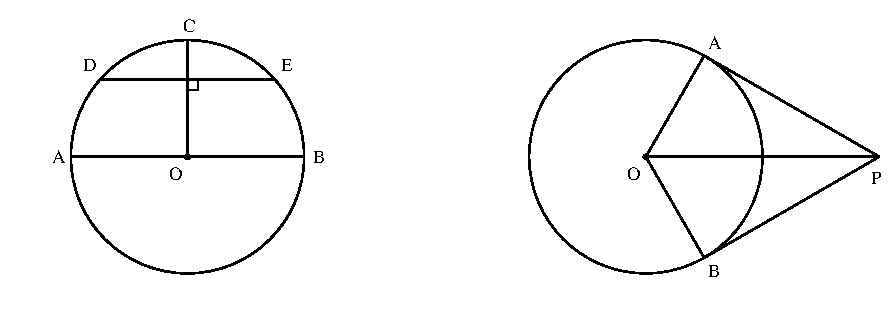
\includegraphics[width=\linewidth,height=55mm,keepaspectratio]{lingkaran.pdf}\end{center}
{\small Kiri: diameter \(AB\), jari-jari \(OC\), tali busur \(DE\), dan jarak tegak lurus pusat ke tali busur. Kanan: dua ruas singgung \(PA\) dan \(PB\); gambar ilustratif, bukan ukuran soal.\par}\medskip
\clearpage
\begin{center}\bfseries\large LAMPIRAN 1. ASESMEN AWAL\end{center}\medskip
{\small Nama: \_\_\_\_\_\_\_\_\_\_\_\_\_\_\_\_\_\_\_\_\_\_\_\_\_\_\_\_\_\_\_\_\_\_  Kelas: \_\_\_\_\_\_\_\_\_\_\par}\medskip
{\small Waktu rencana: 30 menit. Kerjakan mandiri, sertakan langkah dan alasan; gunakan lembar tambahan atau sketsa bila perlu.\par}\medskip
\noindent\textbf{D1 / TP1.} Gambarlah lingkaran berpusat \(O\) dengan diameter \(AB=14\) cm. Tambahkan tali busur \(CD\) yang tidak melalui pusat, satu busur, juring, dan apotema terhadap \(CD\). Tentukan jari-jari dan jelaskan perbedaan diameter dengan tali busur.\par\vspace{10mm}
\noindent\textbf{D2 / TP2.} Sudut pusat yang menghadap busur \(AB\) adalah \(100^\circ\). Titik \(C\) terletak pada busur pelengkap. Tentukan \(\angle ACB\). Pada segiempat siklik \(KLMN\), jika sudut \(K=70^\circ\), berapa sudut \(M\)? Jelaskan.\par\vspace{10mm}
\noindent\textbf{D3 / TP3.} Jari-jari lingkaran 13 cm dan jarak tegak lurus pusat ke tali busur 5 cm. Buat sketsa dan hitung panjang tali busur.\par\vspace{10mm}
\noindent\textbf{D4 / TP4.} Titik \(P\) berjarak 13 cm dari pusat lingkaran berjari-jari 5 cm. Dua garis dari \(P\) menyinggung lingkaran di \(A\) dan \(B\). Hitung \(PA\) dan \(PB\), serta jelaskan alasannya.\par\vspace{10mm}
\noindent\textbf{D5 / TP5.} Taman berbentuk lingkaran berjari-jari 14 m. Jalur dan bidang hias membentuk juring \(90^\circ\). Tentukan panjang busur dan luas juring; gunakan \(\pi=\frac{22}{7}\). Jelaskan asumsi bentuk taman.\par\vspace{10mm}
{\small Guru mengonfirmasi pemahaman lewat pertanyaan lisan bila bukti tertulis belum cukup. Kelompok layanan dibentuk per TP dan dapat berubah mengikuti kemajuan.\par}\medskip
\clearpage
\begin{center}\bfseries\large D. RENCANA PROGRAM REMEDIAL\end{center}\medskip
Peserta adalah murid dengan bukti TP level 1-2. Satu siklus direncanakan 3 pertemuan × 2 JP, hanya untuk kompetensi yang masih memerlukan bantuan. Durasi disesuaikan perkembangan peserta.\par\medskip
{\small\setlength{\tabcolsep}{2mm}\renewcommand{\arraystretch}{1.35}\begin{longtable}{|>{\raggedright\arraybackslash}p{16.847mm}|>{\raggedright\arraybackslash}p{89.049mm}|>{\raggedright\arraybackslash}p{16.847mm}|>{\raggedright\arraybackslash}p{38.507mm}|}\hline
\rowcolor{gray!10}\textbf{Sesi} & \textbf{Kegiatan pendampingan} & \textbf{Waktu} & \textbf{Bukti kemajuan}\\ \hline
\endfirsthead
\rowcolor{gray!10}\textbf{Sesi} & \textbf{Kegiatan pendampingan} & \textbf{Waktu} & \textbf{Bukti kemajuan}\\ \hline
\endhead
R1\newline TP1-TP2 & Memahami: wawancara kesalahan (15 menit). Mengaplikasi: contoh terurai dan latihan terbimbing (35 menit), latihan mandiri (30 menit). Merefleksi: tiket keluar (10 menit). Sketsa berwarna, penandaan busur, dan perbandingan sudut pada busur sama. & 2 JP\newline 90 menit & Catat alasan, hasil, bantuan yang masih diperlukan, dan level TP terbaru.\\ \hline
R2\newline TP3-TP4 & Memahami: wawancara kesalahan (15 menit). Mengaplikasi: contoh terurai dan latihan terbimbing (35 menit), latihan mandiri (30 menit). Merefleksi: tiket keluar (10 menit). Segitiga siku-siku bantu, jarak tegak lurus, serta pembuktian dua ruas singgung. & 2 JP\newline 90 menit & Catat alasan, hasil, bantuan yang masih diperlukan, dan level TP terbaru.\\ \hline
R3\newline TP5 & Memahami: identifikasi model (15 menit). Mengaplikasi: latihan terarah (20 menit), asesmen ulang TP sasaran (40 menit). Merefleksi: umpan balik dan tindak lanjut (15 menit). Model taman, perbandingan alternatif panjang/luas, dan pemeriksaan satuan serta asumsi. & 2 JP\newline 90 menit & Catat alasan, hasil, bantuan yang masih diperlukan, dan level TP terbaru.\\ \hline
\end{longtable}}\medskip
\par\medskip\noindent\textbf{Dukungan dan nilai pembelajaran}\par\smallskip
Gunakan tabel, sketsa, kartu konsep, serta contoh konkret. Guru memodelkan cara berpikir lalu mengurangi bantuan. Tutor sebaya mendukung diskusi dan tidak menggantikan pendampingan guru. Sediakan lembar cetak, instruksi yang mudah dibaca, tambahan waktu atau jawaban lisan sesuai kebutuhan.\par\medskip
{\small Cinta ilmu diwujudkan melalui ketelitian dan kejujuran pemeriksaan; cinta diri dan sesama melalui bantuan tanpa mempermalukan kesalahan. Konteks tanaman atau taman menumbuhkan kepedulian lingkungan.\par}\medskip
\par\medskip\noindent\textbf{Keputusan setelah layanan}\par\smallskip
{\small TP level 3 kembali ke kegiatan reguler atau mendapat pengayaan. Jika belum tercapai, ubah bantuan dan jadwalkan siklus singkat berikutnya. Simpan bukti awal, lembar kerja, asesmen ulang, dan umpan balik. Pelaporan nilai mengikuti kebijakan madrasah tanpa pembatasan otomatis nilai remedial dalam program ini.\par}\medskip
\clearpage
\begin{center}\bfseries\large LAMPIRAN 2. LEMBAR KERJA REMEDIAL\end{center}\medskip
{\small Nama: \_\_\_\_\_\_\_\_\_\_\_\_\_\_\_\_\_\_\_\_\_\_\_\_\_\_\_\_\_\_\_\_\_\_  Kelas: \_\_\_\_\_\_\_\_\_\_\par}\medskip
{\small Guru memilih butir sesuai TP sasaran. Jelaskan alasan pemilihan rumus dan tunjukkan pemeriksaan hasil.\par}\medskip
\noindent\textbf{R1 / TP1.} Gambar lingkaran dengan diameter 20 cm. Tandai pusat, dua jari-jari, diameter, tali busur lain, busur, juring, dan apotema. Hitung jari-jari dan jelaskan unsur yang melalui pusat.\par\vspace{10mm}
\noindent\textbf{R2 / TP2.} Sudut pusat untuk busur \(AB\) adalah \(120^\circ\). Tentukan sudut keliling pada busur yang sama. Jika satu sudut segiempat siklik \(85^\circ\), tentukan sudut berhadapannya.\par\vspace{10mm}
\noindent\textbf{R3 / TP3.} Lingkaran berjari-jari 10 cm memiliki tali busur berjarak 6 cm dari pusat. Gambarkan segitiga bantu, hitung setengah tali busur, kemudian panjang seluruh tali busur.\par\vspace{10mm}
\noindent\textbf{R4 / TP4.} Titik luar \(P\) berjarak 10 cm dari pusat, sedangkan jari-jari 6 cm. Hitung panjang ruas singgung. Tunjukkan sudut siku-siku dan jelaskan kesamaan dua ruas singgung dari \(P\).\par\vspace{10mm}
\noindent\textbf{R5 / TP5.} Sebuah juring berjari-jari 7 m memiliki sudut pusat \(120^\circ\). Hitung panjang busur dan luasnya dalam bentuk eksak memuat \(\pi\). Bandingkan panjang busur dengan keliling lingkaran penuh.\par\vspace{10mm}
{\small Kesalahan yang saya perbaiki: \_\_\_\_\_\_\_\_\_\_\_\_\_\_\_\_\_\_\_\_\_\_\_\_\_\_\_\_\_\_\_\_\_\_\_\_\_\_\_\_\newline Cara saya memeriksa jawaban: \_\_\_\_\_\_\_\_\_\_\_\_\_\_\_\_\_\_\_\_\_\_\_\_\_\_\_\_\_\_\_\_\_\_\_\_\_\_\_\_\_\par}\medskip
\clearpage
\begin{center}\bfseries\large LAMPIRAN 3. ASESMEN ULANG\end{center}\medskip
{\small Nama: \_\_\_\_\_\_\_\_\_\_\_\_\_\_\_\_\_\_\_\_\_\_\_\_\_\_\_\_\_\_\_\_\_\_  Kelas: \_\_\_\_\_\_\_\_\_\_\par}\medskip
{\small Waktu rencana: 40 menit. Kerjakan mandiri; asesmen dipilih sesuai TP sasaran remedial.\par}\medskip
\noindent\textbf{U1 / TP1.} Gambar lingkaran dengan diameter 18 cm. Tentukan jari-jari dan tandai pusat, diameter, tali busur yang bukan diameter, busur, juring, serta apotema. Jelaskan satu hubungan antarunsur.\par\vspace{10mm}
\noindent\textbf{U2 / TP2.} Sudut pusat untuk busur \(AB\) adalah \(140^\circ\). Tentukan sudut keliling pada busur yang sama. Pada segiempat siklik, satu sudut \(115^\circ\); tentukan sudut berhadapannya.\par\vspace{10mm}
\noindent\textbf{U3 / TP3.} Jari-jari lingkaran 17 cm dan jarak tegak lurus pusat ke tali busur 8 cm. Tentukan panjang tali busur dan jelaskan segitiga yang digunakan.\par\vspace{10mm}
\noindent\textbf{U4 / TP4.} Titik \(P\) berjarak 25 cm dari pusat lingkaran berjari-jari 7 cm. Hitung panjang kedua ruas singgung dari \(P\); jelaskan hubungan jari-jari dan garis singgung.\par\vspace{10mm}
\noindent\textbf{U5 / TP5.} Sebuah juring berjari-jari 21 m bersudut pusat \(60^\circ\). Tentukan panjang busur dan luas juring dengan \(\pi=\frac{22}{7}\), lengkap dengan satuan serta pemeriksaan kewajaran.\par\vspace{10mm}
{\small Penetapan hasil memakai rubrik bagian B. TP tercapai ketika seluruh bukti esensialnya tampak mandiri minimal level 3. Periksa konsep, alasan, satuan, dan kewajaran hasil.\par}\medskip
\clearpage
\begin{center}\bfseries\large E. RENCANA PROGRAM PENGAYAAN\end{center}\medskip
Peserta telah mencapai minimal level 3 pada TP sasaran. Pilih satu proyek; peserta tetap menjelaskan kontribusi dan pemikirannya sendiri. Pengayaan memperluas pemodelan dan penalaran, tidak sekadar menambah soal sejenis.\par\medskip
{\small\setlength{\tabcolsep}{2mm}\renewcommand{\arraystretch}{1.35}\begin{longtable}{|>{\raggedright\arraybackslash}p{15.752mm}|>{\raggedright\arraybackslash}p{112.892mm}|>{\raggedright\arraybackslash}p{36.756mm}|}\hline
\rowcolor{gray!10}\textbf{Sesi} & \textbf{Aktivitas} & \textbf{Waktu / produk}\\ \hline
\endfirsthead
\rowcolor{gray!10}\textbf{Sesi} & \textbf{Aktivitas} & \textbf{Waktu / produk}\\ \hline
\endhead
P1 & Pilih konteks dan nyatakan asumsi (15 menit); eksplorasi rumus/tabel/sketsa (60 menit); pemeriksaan dan refleksi (15 menit). & 2 JP / 90 menit\newline Draf solusi dan bukti pemeriksaan.\\ \hline
P2 & Perbaiki model berdasar umpan balik (35 menit); presentasi serta verifikasi individual (35 menit); evaluasi keterbatasan (20 menit). & 2 JP / 90 menit\newline Laporan 1-2 halaman dan refleksi individual.\\ \hline
\end{longtable}}\medskip
\par\medskip\noindent\textbf{Proyek A - Memilih jalur taman}\par\smallskip
Dua titik \(A\) dan \(B\) pada taman lingkaran berjari-jari 14 m membentuk sudut pusat \(90^\circ\). Bandingkan jalur busur pendek dengan jalur lurus tali busur. Hitung panjang keduanya, selisihnya, jarak pusat ke tali busur, dan tinggi tembereng di tengah. Beri rekomendasi dengan mempertimbangkan jarak serta ruang hijau; nyatakan asumsi dan sketsa berskala.\par\medskip
\par\medskip\noindent\textbf{Proyek B - Membuktikan hubungan dua garis singgung}\par\smallskip
Lingkaran berpusat \(O\) berjari-jari 5 cm; \(OP=10\) cm. Dua ruas dari \(P\) menyinggung di \(A\) dan \(B\). Buktikan \(PA=PB\) menggunakan segitiga siku-siku. Hitung panjang keduanya, sudut pusat minor \(\angle AOB\), dan sudut \(\angle APB\). Jelaskan mengapa kedua sudut terakhir berjumlah \(180^\circ\) dan verifikasi lewat gambar.\par\medskip
{\small Produk memuat masalah, variabel/unsur, rumus, tabel atau sketsa, pemeriksaan, kesimpulan, dan batas model. Gunakan data soal sebagai simulasi; data nyata hanya dicantumkan bila benar-benar diperoleh.\par}\medskip
\clearpage
\begin{center}\bfseries\large F. RUBRIK PENGAYAAN DAN REFLEKSI\end{center}\medskip
{\small\setlength{\tabcolsep}{2mm}\renewcommand{\arraystretch}{1.35}\begin{longtable}{|>{\raggedright\arraybackslash}p{27.873mm}|>{\raggedright\arraybackslash}p{26.606mm}|>{\raggedright\arraybackslash}p{29.140mm}|>{\raggedright\arraybackslash}p{35.474mm}|>{\raggedright\arraybackslash}p{38.008mm}|}\hline
\rowcolor{gray!10}\textbf{Aspek} & \textbf{Level 1} & \textbf{Level 2} & \textbf{Level 3} & \textbf{Level 4}\\ \hline
\endfirsthead
\rowcolor{gray!10}\textbf{Aspek} & \textbf{Level 1} & \textbf{Level 2} & \textbf{Level 3} & \textbf{Level 4}\\ \hline
\endhead
Model / representasi & Belum sesuai konteks. & Sebagian sesuai; asumsi belum jelas. & Model dan representasi tepat serta beralasan. & Menguji batas atau memberi alternatif yang sah.\\ \hline
Prosedur / argumen & Langkah utama belum benar. & Memerlukan arahan pada langkah utama. & Perhitungan serta alasan runtut dan mandiri. & Memberi generalisasi atau pemeriksaan berbeda.\\ \hline
Evaluasi konteks & Belum menafsirkan hasil. & Tafsiran sebagian sesuai. & Kesimpulan wajar; satuan dan asumsi jelas. & Menguji keterbatasan dan memberi usul validasi.\\ \hline
Komunikasi individual & Belum menjelaskan kontribusi. & Bergantung pada pasangan. & Menjelaskan kontribusi dan alasan sendiri. & Menanggapi sanggahan serta memperbaiki penjelasan.\\ \hline
\end{longtable}}\medskip
{\small Target produk: minimal level 3 pada keempat aspek. Skala ditetapkan guru untuk tugas ini. Penilaian kelompok dilengkapi verifikasi individual; kerja sama diberi umpan balik dan tidak menggantikan bukti matematika.\par}\medskip
\par\medskip\noindent\textbf{Refleksi murid}\par\smallskip
\noindent\textbf{1.} Konsep apa yang membantu saya memilih rumus atau hubungan?\par\vspace{6mm}
\noindent\textbf{2.} Bagaimana saya memeriksa indeks, satuan, atau unsur pada sketsa?\par\vspace{6mm}
\noindent\textbf{3.} Asumsi apa yang membatasi penggunaan hasil?\par\vspace{6mm}
\noindent\textbf{4.} Bantuan dan langkah belajar berikutnya apa yang saya perlukan?\par\vspace{6mm}
\par\medskip\noindent\textbf{Refleksi guru}\par\smallskip
{\small Kesulitan yang masih muncul: \_\_\_\_\_\_\_\_\_\_\_\_\_\_\_\_\_\_\_\_\_\_\_\_\_\_\_\_\_\_\_\_\_\_\_\_\_\_\_\_\_\newline Bantuan yang efektif dan buktinya: \_\_\_\_\_\_\_\_\_\_\_\_\_\_\_\_\_\_\_\_\_\_\_\_\_\_\_\_\_\_\_\_\_\_\_\_\_\newline Perubahan untuk siklus berikutnya: \_\_\_\_\_\_\_\_\_\_\_\_\_\_\_\_\_\_\_\_\_\_\_\_\_\_\_\_\_\_\_\_\_\_\_\_\par}\medskip
\clearpage
\begin{center}\bfseries\large LAMPIRAN 4. KUNCI ASESMEN AWAL\\[2pt] DAN LEMBAR KERJA REMEDIAL\end{center}\medskip
{\small\setlength{\tabcolsep}{2mm}\renewcommand{\arraystretch}{1.35}\begin{longtable}{|>{\raggedright\arraybackslash}p{14.685mm}|>{\raggedright\arraybackslash}p{154.865mm}|}\hline
\rowcolor{gray!10}\textbf{Butir} & \textbf{Jawaban dan bukti yang diperiksa}\\ \hline
\endfirsthead
\rowcolor{gray!10}\textbf{Butir} & \textbf{Jawaban dan bukti yang diperiksa}\\ \hline
\endhead
D1 & \(r=7\) cm. Diameter adalah tali busur yang melalui pusat. Apotema tegak lurus tali busur; juring dibatasi dua jari-jari dan sebuah busur. Periksa penandaan pada sketsa.\\ \hline
D2 & \(\angle ACB=50^\circ\) karena menghadap busur yang sama. Sudut \(M=110^\circ\) karena berhadapan dengan \(K\) pada segiempat siklik.\\ \hline
D3 & Setengah tali busur \(=\sqrt{13^2-5^2}=12\) cm, sehingga panjangnya 24 cm. Garis dari pusat yang tegak lurus tali busur membaginya sama panjang.\\ \hline
D4 & \(PA=PB=\sqrt{13^2-5^2}=12\) cm. Segitiga \(OAP\) siku-siku di \(A\) dan kedua ruas singgung dari \(P\) sama panjang.\\ \hline
D5 & \(s=\frac{90}{360}\cdot2\pi(14)=7\pi=22\) m; \(L=\frac{90}{360}\pi(14)^2=49\pi=154\) m\(^2\). Bentuk diasumsikan lingkaran sempurna.\\ \hline
R1 & \(r=10\) cm. Pusat terletak pada diameter; tali busur lain dapat tidak melalui pusat. Periksa unsur dan apotema pada gambar murid.\\ \hline
R2 & Sudut keliling \(60^\circ\); sudut berhadapan \(95^\circ\). Busur yang dihadapi harus sama pada hubungan sudut pusat-keliling.\\ \hline
R3 & Setengah tali busur \(=\sqrt{10^2-6^2}=8\) cm; panjang seluruhnya 16 cm.\\ \hline
R4 & Ruas singgung \(=\sqrt{10^2-6^2}=8\) cm. Jari-jari tegak lurus di titik singgung; kedua ruas dari titik luar sama panjang.\\ \hline
R5 & \(s=\frac{14\pi}{3}\) m; \(L=\frac{49\pi}{3}\) m\(^2\). Panjang busur adalah sepertiga keliling karena sudutnya sepertiga putaran penuh.\\ \hline
\end{longtable}}\medskip
{\small Jawaban ekuivalen diterima jika langkah dan alasan sah. Kunci membantu pemeriksaan; level TP tetap ditentukan dengan memperhatikan seluruh bukti esensial dan kemandirian.\par}\medskip
\clearpage
\begin{center}\bfseries\large LAMPIRAN 5. KUNCI ASESMEN ULANG\\[2pt] DAN PENGAYAAN\end{center}\medskip
{\small\setlength{\tabcolsep}{2mm}\renewcommand{\arraystretch}{1.35}\begin{longtable}{|>{\raggedright\arraybackslash}p{31.791mm}|>{\raggedright\arraybackslash}p{137.759mm}|}\hline
\rowcolor{gray!10}\textbf{Butir} & \textbf{Jawaban / panduan pemeriksaan}\\ \hline
\endfirsthead
\rowcolor{gray!10}\textbf{Butir} & \textbf{Jawaban / panduan pemeriksaan}\\ \hline
\endhead
U1 & \(r=9\) cm. Periksa pusat, jari-jari, diameter, tali busur, busur, juring, apotema, dan alasan hubungan pada sketsa.\\ \hline
U2 & Sudut keliling \(70^\circ\); sudut berhadapan \(65^\circ\).\\ \hline
U3 & Setengah tali busur \(=\sqrt{17^2-8^2}=15\) cm; panjang seluruhnya 30 cm.\\ \hline
U4 & \(PA=PB=\sqrt{25^2-7^2}=24\) cm; jari-jari tegak lurus garis singgung di titik singgung.\\ \hline
U5 & \(s=\frac{60}{360}\cdot2\pi(21)=7\pi=22\) m; \(L=\frac{60}{360}\pi(21)^2=\frac{147\pi}{2}=231\) m\(^2\). Keduanya seperenam besaran lingkaran penuh.\\ \hline
Proyek A: panjang & Busur pendek \(7\pi\) m; tali busur \(14\sqrt2\) m. Selisih \(7\pi-14\sqrt2\) m. Jika memakai \(\pi\approx3{,}14159\), selisih sekitar 2,192 m; busur lebih panjang.\\ \hline
Proyek A: jarak & Jarak pusat ke tali busur \(7\sqrt2\) m; tinggi tembereng tengah \(14-7\sqrt2\) m. Rekomendasi harus memperhitungkan ruang hijau dan akses, tidak hanya hasil hitungan.\\ \hline
Proyek B & \(PA=PB=5\sqrt3\) cm. Segitiga \(OAP\) dan \(OBP\) kongruen karena siku-siku, sisi miring \(OP\) sama, dan \(OA=OB\). Diperoleh \(\angle AOP=\angle POB=60^\circ\), sehingga sudut pusat minor \(120^\circ\) dan \(\angle APB=60^\circ\). Dua sudut siku-siku pada segiempat \(OAPB\) membuat jumlah dua sudut lainnya \(180^\circ\).\\ \hline
\end{longtable}}\medskip
\clearpage
\begin{center}\bfseries\large LAMPIRAN 6. FORMAT PELAKSANAAN\\[2pt] DAN TINDAK LANJUT\end{center}\medskip
\par\medskip\noindent\textbf{1. Pemetaan dan keputusan per peserta}\par\smallskip
{\small\setlength{\tabcolsep}{2mm}\renewcommand{\arraystretch}{1.35}\begin{longtable}{|>{\raggedright\arraybackslash}p{10.030mm}|>{\raggedright\arraybackslash}p{37.611mm}|>{\raggedright\arraybackslash}p{20.059mm}|>{\raggedright\arraybackslash}p{17.552mm}|>{\raggedright\arraybackslash}p{22.566mm}|>{\raggedright\arraybackslash}p{45.133mm}|}\hline
\rowcolor{gray!10}\textbf{No} & \textbf{Nama / kelas} & \textbf{TP sasaran} & \textbf{Level awal} & \textbf{Layanan} & \textbf{Level akhir / tindak lanjut}\\ \hline
\endfirsthead
\rowcolor{gray!10}\textbf{No} & \textbf{Nama / kelas} & \textbf{TP sasaran} & \textbf{Level awal} & \textbf{Layanan} & \textbf{Level akhir / tindak lanjut}\\ \hline
\endhead
1 & \rule{0pt}{8mm} &  &  &  & \\ \hline
2 & \rule{0pt}{8mm} &  &  &  & \\ \hline
3 & \rule{0pt}{8mm} &  &  &  & \\ \hline
4 & \rule{0pt}{8mm} &  &  &  & \\ \hline
5 & \rule{0pt}{8mm} &  &  &  & \\ \hline
6 & \rule{0pt}{8mm} &  &  &  & \\ \hline
\end{longtable}}\medskip
\par\medskip\noindent\textbf{2. Jurnal kegiatan}\par\smallskip
{\small\setlength{\tabcolsep}{2mm}\renewcommand{\arraystretch}{1.35}\begin{longtable}{|>{\raggedright\arraybackslash}p{26.434mm}|>{\raggedright\arraybackslash}p{29.078mm}|>{\raggedright\arraybackslash}p{47.582mm}|>{\raggedright\arraybackslash}p{58.156mm}|}\hline
\rowcolor{gray!10}\textbf{Tanggal / JP} & \textbf{TP / kelompok} & \textbf{Bantuan atau tugas} & \textbf{Bukti belajar / umpan balik}\\ \hline
\endfirsthead
\rowcolor{gray!10}\textbf{Tanggal / JP} & \textbf{TP / kelompok} & \textbf{Bantuan atau tugas} & \textbf{Bukti belajar / umpan balik}\\ \hline
\endhead
\rule{0pt}{8mm} &  &  & \\ \hline
\rule{0pt}{8mm} &  &  & \\ \hline
\rule{0pt}{8mm} &  &  & \\ \hline
\end{longtable}}\medskip
\par\medskip\noindent\textbf{3. Evaluasi program}\par\smallskip
{\small\setlength{\tabcolsep}{2mm}\renewcommand{\arraystretch}{1.35}\begin{longtable}{|>{\raggedright\arraybackslash}p{77.826mm}|>{\raggedright\arraybackslash}p{91.724mm}|}\hline
Jumlah peserta remedial / pengayaan & \_\_\_\_\_\_\_\_\_\_\_\_ / \_\_\_\_\_\_\_\_\_\_\_\_\\ \hline
TP tercapai setelah layanan & \_\_\_\_\_\_\_\_\_\_\_\_\_\_\_\_\_\_\_\_\_\_\_\_\_\_\_\_\_\_\_\_\\ \hline
TP masih perlu dukungan & \_\_\_\_\_\_\_\_\_\_\_\_\_\_\_\_\_\_\_\_\_\_\_\_\_\_\_\_\_\_\_\_\\ \hline
Tindak lanjut dan jadwal berikutnya & \_\_\_\_\_\_\_\_\_\_\_\_\_\_\_\_\_\_\_\_\_\_\_\_\_\_\_\_\_\_\_\_\\ \hline
Dokumen bukti & Asesmen awal, lembar kerja, asesmen ulang, produk, rubrik, dan umpan balik.\\ \hline
\end{longtable}}\medskip
{\small Diisi setelah kegiatan berdasarkan bukti nyata; kehadiran atau selesainya tugas tidak menggantikan bukti ketercapaian kompetensi.\par}\medskip
\clearpage
\begin{center}\bfseries\large DAFTAR RUJUKAN RESMI\end{center}\medskip
[1] Kementerian Agama. KMA Nomor 1503 Tahun 2025 tentang perubahan atas KMA Nomor 450 Tahun 2024; terutama Bab IV Pembelajaran dan Asesmen.\par\medskip
\href{https://sulteng.kemenag.go.id/files/show/20251020162801surat-penyampaian-kma-kurikulum-2025%2Blampiran_compressed-tzR.pdf}{\small\textcolor{blue}{Buka sumber resmi}}\par
\vspace{8.50393701pt}
[2] Permendikdasmen Nomor 13 Tahun 2025 tentang perubahan ketentuan kurikulum; tercantum dalam dasar hukum Keputusan Kepala BSKAP 046/H/KR/2025.\par\medskip
\href{https://bpmpbabel.kemendikdasmen.go.id/PPID/wp-content/uploads/2025/07/KepKaBSKAP-046_2025-ttg-CP.pdf}{\small\textcolor{blue}{Buka sumber resmi}}\par
\vspace{8.50393701pt}
[3] Kemendikdasmen. Abstrak resmi Permendikdasmen Nomor 1 Tahun 2026 tentang Standar Proses. Berlaku 5 Januari 2026 dan menggantikan standar proses tahun 2022.\par\medskip
\href{https://jdih.kemendikdasmen.go.id/sjdih/siperpu/dokumen/abstraksi/Abstrak%20RPM%20Standar%20Proses.pdf}{\small\textcolor{blue}{Buka sumber resmi}}\par
\vspace{8.50393701pt}
[4] Pusat Standar dan Kebijakan Pendidikan. Laman Standar Nasional Pendidikan, bagian Standar Penilaian; memuat rujukan Permendikbudristek Nomor 21 Tahun 2022.\par\medskip
\href{https://pskp.kemendikdasmen.go.id/standar-nasional-pendidikan-a/standar-proses}{\small\textcolor{blue}{Buka sumber resmi}}\par
\vspace{8.50393701pt}
[5] Keputusan Kepala BSKAP Nomor 046/H/KR/2025. Lampiran II, Matematika, Fase F, elemen 6.3 Geometri.\par\medskip
\href{https://bpmpbabel.kemendikdasmen.go.id/PPID/wp-content/uploads/2025/07/KepKaBSKAP-046_2025-ttg-CP.pdf}{\small\textcolor{blue}{Buka sumber resmi}}\par
\vspace{8.50393701pt}
[6] Kemendikdasmen. Panduan Pembelajaran dan Asesmen, Edisi Revisi 2025. Bagian kriteria ketercapaian, remedial, pengayaan, dan pengolahan hasil asesmen.\par\medskip
\href{https://kurikulum.kemendikdasmen.go.id/file/1755668120_manage_file.pdf}{\small\textcolor{blue}{Buka sumber resmi}}\par
\vspace{8.50393701pt}
[7] Kemendikdasmen. Siaran pers 23 Juni 2026 tentang ruang lingkup pembaruan CP melalui Keputusan Kepala BKPDM Nomor 020 Tahun 2026.\par\medskip
\href{https://www.kemendikdasmen.go.id/siaran-pers/15636-capaian-pembelajaran-baru-telah-terbit-yang-berubah-hanya-mata-pelajaran-agama-dan-budi-pekerti}{\small\textcolor{blue}{Buka sumber resmi}}\par
\vspace{8.50393701pt}
{\small Pemeriksaan sumber: 31 Oktober 2026. Rencana waktu, perangkat tugas, rubrik, dan format administrasi dalam program ini disusun untuk kebutuhan unit oleh guru dan dapat diselaraskan dengan ATP serta kebijakan penilaian madrasah.\par}\medskip
\end{document}
